\section{Background}
\label{sec:background}

\input{tim/science1}

 

\subsection{Static Code Analysis}
Automatic static analysis (SA) tools, such as Findbugs
%(see Figure~\ref{fig:fb}), 
are tools for   detecting bugs in source code,
without having to execute that code.
As they can find real bugs at low cost~\cite{thung2012extent,habib2018many}, they have been adopted in open source projects and in industry~\cite{ayewah2010google,sadowski2018lessons,beller2016analyzing,zampetti2017open,panichella2015would,vassallo2020developers}.
However, as they do not guarantee that all warnings are real bugs, 
these tools produce false alarms. 
The large number of false alarms produced is a barrier to adoption~\cite{johnson2013don,ChristakisB16}; it is easy to imagine how developers will be frustrated by using tools that require them to inspect numerous false alarms before finding a real bug.
While false alarms include spurious warnings caused by the over-approximation of possible program behaviors during program analysis, 
false alarms also refer to warnings that developers do not act on.
For example, developers may not think that the warning represents a bug (e.g. due to ``style'' warnings that developers perceive to be of little benefit) or may not wish to modify obsolete code. 

The problem of addressing false alarms from static analysis tools has been widely studied.
There have been many recent attempts to address the problem. 
Some researchers have proposed new SA tools that use  more sophisticated, but costly, static analysis techniques (e.g. Infer~\cite{calcagno2015moving}, NullAway~\cite{banerjee2019nullaway}).
Despite their improvements, these tools still produce many false alarms~\cite{tomassi2021real}.
Other attempts to prune false alarms include the use of test case generation to validate the presence of a bug  at the source code location indicated by the warning~\cite{kallingal2021validating}.
As generating test cases is expensive, these techniques may face issues when scaling up to larger projects, limiting their practicality.


\subsection{Early Results:  Wang et al., 2018}


By framing the problem as a binary classification problem, 
  machine learning techniques can identify actionable warnings 
  (allowing us to prune false alarms)~\cite{hanam2014finding,heckman2008establishing,liang2010automatic,ruthruff2008predicting,wang2018there,yang2021learning,yang2021understanding}.
These techniques use features extracted from code analysis and metrics computed over the code and warning's history in the project.
Figure \ref{fig:workflow} illustrates this process. 
A static analyzer is ran on a training revision and the warnings produced are labelled. 
When applied to the latest revision, only warnings classified as actionable warnings by the machine learner are presented to the developers.

\begin{figure}[t]
  
  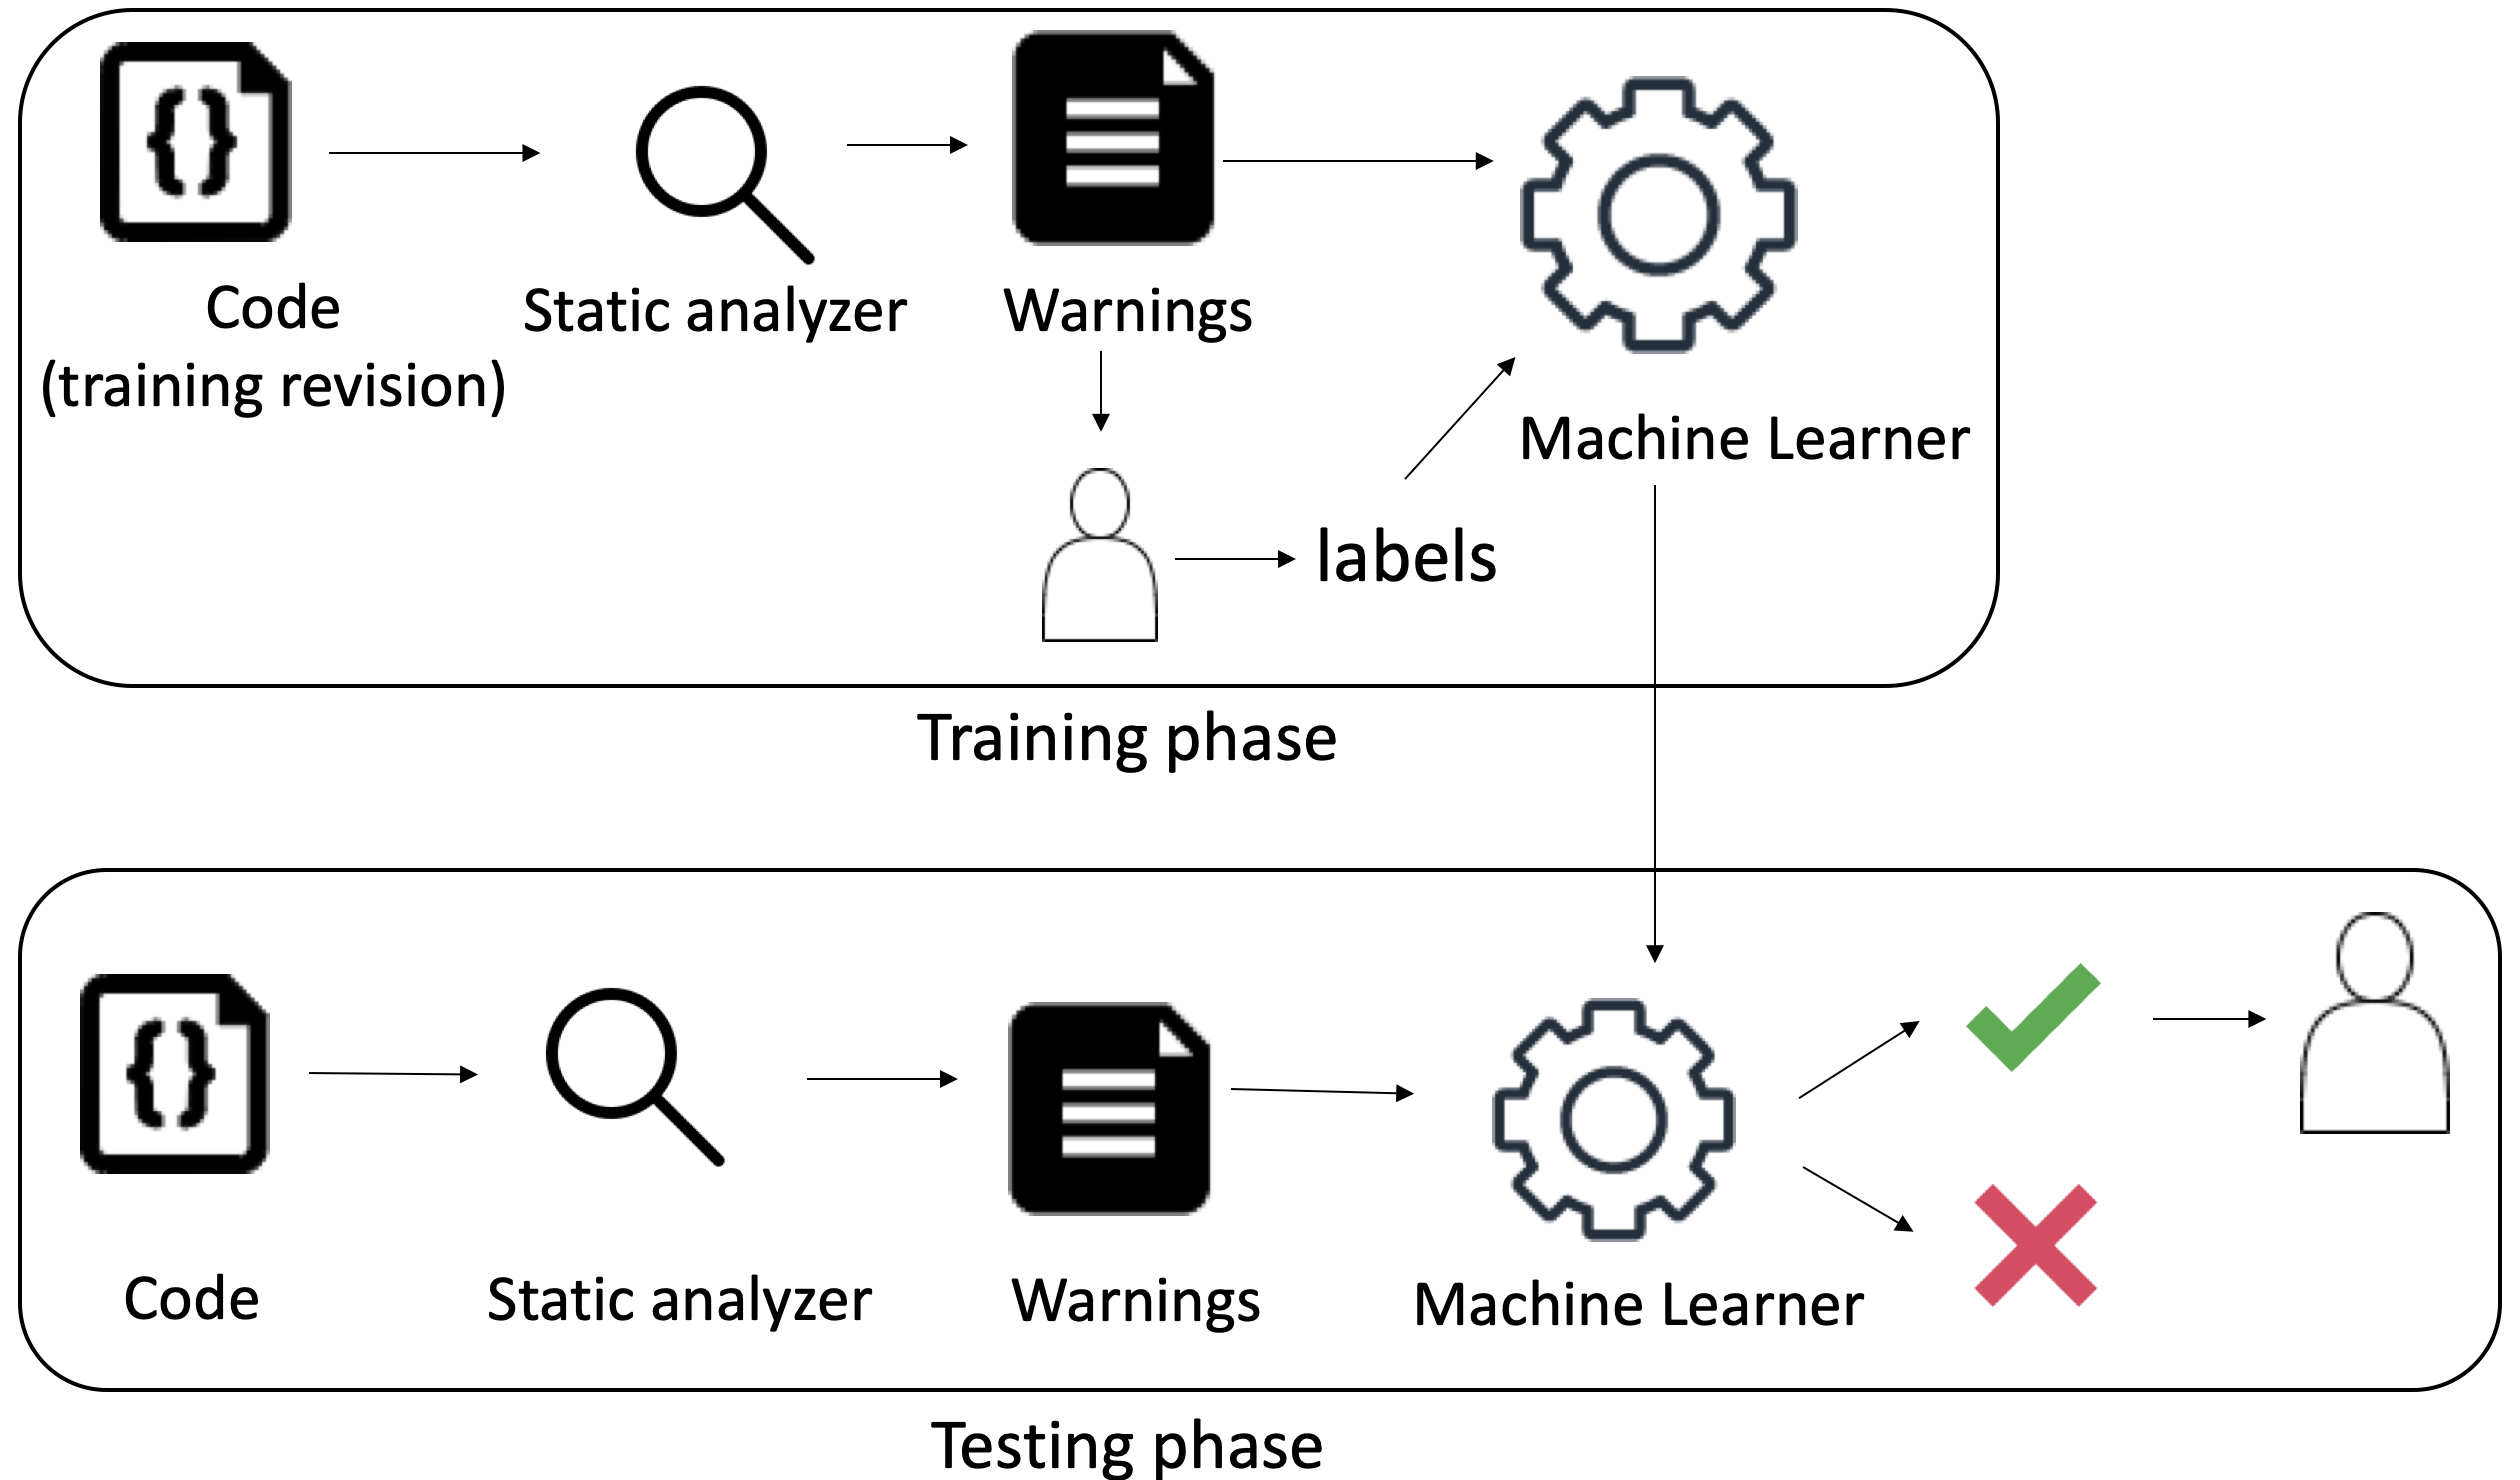
\includegraphics[width=\columnwidth]{hongjin/workflow.png}
  \caption{To detect actionable warnings, a   learner is trained   on warnings from a training revision. Each warning is annotated with a label. When deployed on the latest revision, only warnings classified as actionable warnings by the machine learner are presented to the developers. }
      \label{fig:workflow}
  \centering
  \end{figure}

To assess proposed machine learners, datasets of warnings produced by Findbugs have been created.
As the ground-truth label of each warning is not known, a heuristic was applied to infer them.
This heuristic compares the warnings reported at a particular revision of the project against a revision set in the future.
If a warning is no longer present, but the file is still present, then the heuristic determines that the warning was fixed. 
As such, the warning is actionable.
Otherwise, if the warning is still present, then the warning is a false alarm.


% \begin{table}[t]
% \footnotesize
%   \centering
%   \caption{The features studied in prior work~\cite{wang2018there,yang2021learning,yang2021understanding}. The ``Golden Features'' are in bold.}
%   \label{tab:golden_features}
  
%     \begin{tabular}{l|l}
%       \toprule
%  \textbf{Feature type}     & \textbf{Feature} \\
%  \midrule
%  & size context for warning type, method  \\ 
%  & size context in file, package \\ 
 
%  & \textbf{warning context in method, file}, package   \\
%  & \textbf{warning context for warning type}  \\
%  & fix, non-fix change removal rate \\
%  Warning  & \textbf{defect likelihood for warning pattern} \\
%  combination & variance of likelihood \\
%  & defect likelihood for warning type \\ 
%  & \textbf{discretization of defect likelihood} \\
%  & \textbf{average lifetime for warning type}\\
%  \midrule
%  & method, file, package size\\
%  & comment length \\
%  & \textbf{comment-code ratio} \\
%  & \textbf{method depth}  \\
%   & \textbf{file depth} \\
%  Code  & method callers, callees \\ 
%  characteristics & \textbf{\# methods in file}, package \\
%  & classes in file \\ 
%  & \textbf{\# classes in package} \\
%  & indentation \\ 
%  & complexity \\
%  \midrule
%  & \textbf{warning pattern} \\
%  & \textbf{warning type}  \\
%  Warning  & \textbf{warning priority}  \\
%  characteristics & warning rank, warnings in method, file \\
%  & \textbf{package} \\
%  \hline
%  & latest file, package modification \\ 
%  & file, package staleness \\
%  File & \textbf{file age, creation}  \\
%  history & deletion revision \\
%  & \textbf{developers} \\
%  \hline
%  & call name, class, \textbf{parameter signature} \\
%  & \textbf{method visibility} \\
%  & return type \\ 
%  & new type, new concrete type \\ 
%  & operator \\ 
%  Code  & field access class, field \\ 
%  analysis & catch \\ 
%  & field name, type, visibility, is static/final \\ 
%  & return type \\ 
%  & is static/ final/ abstract/ protected \\ 
%  & class visibility,is interface \\
%  \hline
%  & added, changed, deleted, growth, total,  \\
%  & percentage of LOC in file (past 3 months) \\
%   & LOC \textbf{added} , changed, deleted, growth \\
%  Code  & total, percentage in file (last 25 revisions)\\
%  history &  \textbf{added}, changed, deleted, growth, total,  \\ 
%  & percentage of LOC in package  (past 3 months) \\
%  & added, changed, deleted, growth, total,  \\
%  & percentage of LOC in package (last 25 revisions) \\
% \hline
% Warning  & \textbf{warning lifetime by revision}, by time \\
% history & warning modifications, open revision \\
% \midrule
% File  & file type, name \\
% Characteristics & package name \\
% \bottomrule 
% \end{tabular}


% \end{table}

 Wang et al.~\cite{wang2018there} ran a systematic literature review to collect  and analyze 100+ features proposed in the literature, categorizing them into 8 categories.
To remove ineffective features, they performed a greedy backward selection algorithm.
From the features, they identified a set of features that     offered effective performance.
% Table \ref{tab:golden_features} lists these features.

\subsection{Further Result: Yang et al., 2021}

Yang et al.~\cite{yang2021learning} further analyzed the   features using the data collected by Wang et al.~\cite{wang2018there}. 
They found that all machine learning techniques were effective and performed similarly to one another. 
Their analysis revealed that the intrinsic dimensionality of the problem was low; 
the features used in the experiments were more verbose than the actual attributes required for classifying actionable warnings.
This motivates the use of simpler machine learners over more complex learners.
From their analysis, SVMs were recommended for use in this problem, as they were both effective and can be trained at a low cost.
In contrast, deep learners were effective but more costly to train.

For each project in their experiments, 
one revision (training revision) was selected for extracting warnings for training the learner, 
and another revision (testing revision) set chronologically in the future of the training revision is selected for extracting warnings for evaluating the learner. 
This simulates a realistic usage scenario of the tool, where the learner is trained using past data before developers apply it to  another revision of the source code.



\subsection{Issues in Prior Results: Kang et al., 2022}
Subsequently, Kang et al.~\cite{kang2022detecting} replicated  the Yang et al.~\cite{yang2021learning} study
to find subtle methodological issues in the     Wang et al. data~\cite{wang2018there} which   led to overoptimistic results.

Firstly, Kang et al. found data leakage where the information regarding the warning in the future, used to determine the ground-truth labels,  leaked into several features.
Five features (warning context in method, file, for warning type, defect likelihood, discretization of defect likelihood) measure the ratio of actionable warnings within a subset of warnings (e.g. warnings in a method, file, of a warning type). 
To determine if a warning is actionable, the ground-truth label was used to compute these features, leading to data leakage.
Kang et al.   reimplemented the features such that they are computed using only historical information, without reference to the ground truth determined from the future state of the projects.
As only the features were reimplemented, the total number of training and testing instances remained unchanged.

Secondly, they found many warnings appearing in both the training and testing dataset. 
As some warnings remain in the project at the time of both the training and testing dataset, the model has access to the ground-truth label for the warning at training time.
Kang et al. addressed this issue by removing warnings that were already present during the training revision from the testing dataset, ensuring that the learner does not see the same warning in both datasets.
After removing these warnings, the number of warnings in the testing revision decreased from
15,695 to 2,615.
% 15,363 to 


\begin{table}[t]
    \centering
    \caption{Evaluation metrics based on TP (true positives); TN (true negatives);
    TP (true positives) and FP (false positives)}
    \label{tab:metrics}
      \rowcolors{2}{white}{gray!15}
    \begin{tabular}{rp{5cm}}
        \toprule
        \textbf{Evaluation Metric} & \textbf{Description}  \\
        \midrule
        Precision & $\frac{\text { TP } }{\text {TP}+\text {FP}}$ \\ 
    
        AUC  & area under the receiver operating
characteristics curve (the true positive
rate against the false positive rate) \\ 
   
        False alarm rate & $\frac{\text { FP } }{\text {FP}+\text {TN}}$\\
      
        Recall &  $\frac{\text { TP } }{\text {TP}+\text {FN}}$ \\
        \bottomrule
    \end{tabular}
\end{table}


\begin{table}[!t]
  \centering
  \caption{The Kang et al. predictors did not perform well on the repaired data. In this table,{\em lower} false alarms are better while {\em higher} precisions, AUC, and recall are {\em better}. }
  \label{tab:initial_svm}
  \rowcolors{2}{white}{gray!15}
  \begin{tabular}{rrrrr}
 
 \toprule
                 
 \textbf{Dataset}           &  \textbf{Precision} & \textbf{AUC} & \textbf{False alarm rate} & \textbf{Recall}          \\
  \midrule 
  cassandra & 0.67 & 0.33 & 0.25 & 0.67 \\
   commons & 0.67 & 0.52 & 0.57 & 0.62 \\
   
  lucene-solr & 0.56 & 0.70  & 0.36 &  0.71\\
  
  median & 0.52 & 0.41 & 0.19 & 0.32 \\
  jmeter & 0.50 & 0.36 & 0.14 & 0.17 \\
  
  tomcat & 0.52 & 0.41 & 0.19 & 0.32 \\
  
  derby & 0.20 & 0.64 & 0.12 & 0.08 \\
 
  ant & 0.00 & 0.00 & 0.00 & 0.00 \\
  \bottomrule
  \end{tabular}
  
\end{table}



Next, Kang et al. analyzed the warning oracle, based on the heuristic comparing warnings at one revision to another revision in the future, used to automatically produce labels for the warnings in the dataset. 
After manual labelling of the actionable warnings, Kang et al. found that only  47\% of warnings automatically labelled actionable were considered by the human annotators to be actionable.
This indicates that the heuristic employed as the warning oracle is not sufficiently reliable for automatically labelling the dataset. 

Kang et al. manually labelled 1,357 warnings. After filtering out duplicates and  uncertain labels, a dataset of 768 warnings remained.
On this dataset, Kang et al. again applied  off-the-shelf SVM models, assessing them with the evaluation metrics listed in Table \ref{tab:metrics}. 




For their reasoning, 
Kang et al. used  the learners recommended by prior work;
i.e. radial bias  SVMs.
The results of the SVM are shown in Table \ref{tab:initial_svm}.
Those results are hardly impressive:
\bi
\item Median precisions barely more than 50\%;
\item Very low median AUCs of 41\%;
\item Extremely low median recalls of 32\%.
\ei
That is to say, while Kang et al. were certainly correct
in their criticisms of the data used in prior work, based on their paper,
it is still an open issue about how to   generate good predictors for static code false alarms. 




% In this paper, we build upon the features identified in the prior studies~\cite{hanam2014finding,heckman2008establishing,liang2010automatic,ruthruff2008predicting,wang2018there,yang2021learning,yang2021understanding}; but instead of only using off-the-shelf machine learners, we tap on the power of more advanced and specialized learners, data engineering methods and hyperparameter optimization steps.


%Another aspect of the analysis addressed by Kang et al.~\cite{kang2022detecting} was the dataset. In particular, they analyzed the heuristic used to infer labels. They found that the labels were inaccurate and were not consistent with manually labelled data by human annotators. Moreover, their experiments suggested that the effectiveness of the machine learners vary with different strategies for inferring labels. This points to the need for human involvement in curating warnings for a benchmark dataset and highlights the importance of data quality. In turn, it highlights the need for methods that can effectively learn from small quantities of human annotated data given the high cost of labelling.

 
 